\let\negmedspace\undefined
\let\negthickspace\undefined
\documentclass[journal,12pt,onecolumn]{IEEEtran}
\usepackage{cite}
\usepackage{amsmath,amssymb,amsfonts,amsthm}
\usepackage{algorithmic}
\usepackage{graphicx}
\graphicspath{{./figs/}}
\usepackage{textcomp}
\usepackage{xcolor}
\usepackage{txfonts}
\usepackage{listings}
\usepackage{enumitem}
\usepackage{mathtools}
\usepackage{gensymb}
\usepackage{comment}
\usepackage{caption}
\usepackage[breaklinks=true]{hyperref}
\usepackage{tkz-euclide} 
\usepackage{listings}
\usepackage{gvv}    
\usepackage{multicol}



\begin{document}
\title{
ASSIGNMENT 3: GATE 2016\\
GG : Geology and Geophysics}
\author{EE25BTECH11003 -Adharvan Kshathriya Bommagani}
\maketitle

\begin{enumerate}

\item The volume of a sphere of diameter 1 unit is \_\_\_\_\_\_\_\_\_ than the volume of a cube of side 1 unit.  

\hfill{\brak{\text{GATE GG 2016}}}  

\begin{multicols}{4}
\begin{enumerate}
\item least
\item less
\item lesser
\item low
\end{enumerate}
\end{multicols}

\item The unruly crowd demanded that the accused be \_\_\_\_\_\_\_\_\_\_ without trial.  

\hfill{\brak{\text{GATE GG 2016}}}  

\begin{multicols}{4}
\begin{enumerate}
\item hanged
\item hanging
\item hankering
\item hung
\end{enumerate}
\end{multicols}

\item Choose the statement(s) where the underlined word is used correctly:  

(i) A prone is a dried plum.  
(ii) He was lying prone on the floor.  
(iii) People who eat a lot of fat are prone to heart disease.  

\hfill{\brak{\text{GATE GG 2016}}}  

\begin{multicols}{2}
\begin{enumerate}
\item (i) and (iii) only
\item (iii) only
\item (i) and (ii) only
\item (ii) and (iii) only
\end{enumerate}
\end{multicols}

\item Fact: If it rains, then the field is wet.  

Read the following statements:  

(i) It rains  \\
(ii) The field is not wet  \\
(iii) The field is wet  \\
(iv) It did not rain  \\

Which one of the options given below is NOT logically possible, based on the given fact?  

\hfill{\brak{\text{GATE GG 2016}}}  

\begin{multicols}{2}
\begin{enumerate}
\item If (iii), then (iv).  
\item If (i), then (iii).  
\item If (i), then (ii).  
\item If (ii), then (iv).  
\end{enumerate}
\end{multicols}

\item A window is made up of a square portion and an equilateral triangle portion above it. The base of the triangular portion coincides with the upper side of the square. If the perimeter of the window is 6 m, the area of the window in m\textsuperscript{2} is \_\_\_\_\_\_\_\_\_.  

\hfill{\brak{\text{GATE GG 2016}}}  

\begin{multicols}{4}
\begin{enumerate}
\item 1.43
\item 2.06
\item 2.68
\item 2.88
\end{enumerate}
\end{multicols}




\newpage

\textbf{Q.6 - Q.10 carry two marks each.}



\item Students taking an exam are divided into two groups, P and Q such that each group has the same number of students. The performance of each of the students in a test was evaluated out of 200 marks. It was observed that the mean of group P was 105, while that of group Q was 85. The standard deviation of group P was 25, while that of group Q was 5. Assuming that the marks were distributed on a normal distribution, which of the following statements will have the highest probability of being TRUE?

\hfill{\brak{\text{GATE GG 2016}}}


\begin{enumerate}
\item No student in group Q scored less marks than any student in group P.
\item No student in group P scored less marks than any student in group Q.
\item Most students of group Q scored marks in a narrower range than students in group P.
\item The median of the marks of group P is 100.
\end{enumerate}




\item A smart city integrates all modes of transport, uses clean energy and promotes sustainable use of resources. It also uses technology to ensure safety and security of the city, something which critics argue, will lead to a surveillance state.

Which of the following can be logically inferred from the above paragraph?

(i) All smart cities encourage the formation of surveillance states. \\
(ii) Surveillance is an integral part of a smart city. \\
(iii) Sustainability and surveillance go hand in hand in a smart city. \\
(iv) There is a perception that smart cities promote surveillance.

\hfill{\brak{\text{GATE GG 2016}}}

\begin{multicols}{2}
\begin{enumerate}
\item (i) and (iv) only
\item (ii) and (iii) only
\item (iv) only
\item (i) only
\end{enumerate}
\end{multicols}

\item Find the missing sequence in the letter series.

B, FH, LNP, \_\_\_\_.

\hfill{\brak{\text{GATE GG 2016}}}

\begin{multicols}{4}
\begin{enumerate}
\item SUWY
\item TUVW
\item TVXZ
\item TWXZ
\end{enumerate}
\end{multicols}

\item The binary operation $\square$ is defined as $a \square b = ab + (a + b)$, where $a$ and $b$ are any two real numbers. The value of the identity element of this operation, defined as the number $x$ such that $a \square x = a$, for any $a$, is \_\_\_\_\_\_.

\hfill{\brak{\text{GATE GG 2016}}}

\begin{multicols}{4}
\begin{enumerate}
\item 0
\item 1
\item 2
\item 10
\end{enumerate}
\end{multicols}

\newpage



\item Which of the following curves represents the function 
$y = \ln\!\left(|e^{|\sin(|x|)|}|\right)$ for $|x| < 2\pi$? 
Here, $x$ represents the abscissa and $y$ represents the ordinate.


\hfill{\brak{\text{GATE GG 2016}}}


\begin{enumerate}
\item 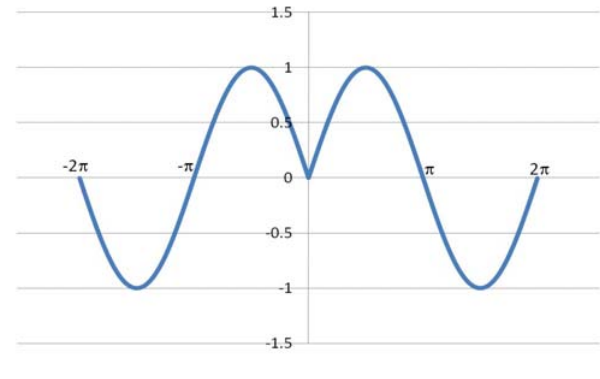
\includegraphics[width=0.5\linewidth]{figs/fig1.png} 
\item 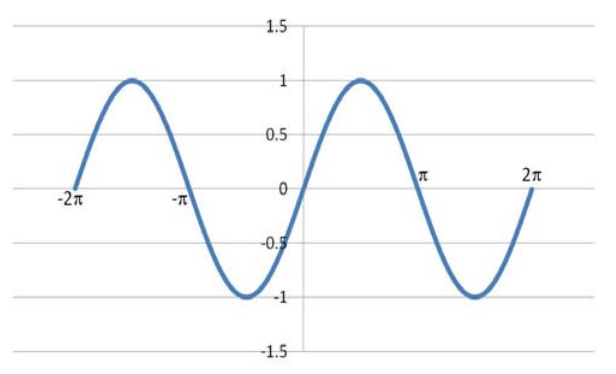
\includegraphics[width=0.5\linewidth]{figs/fig2.png} 
\item 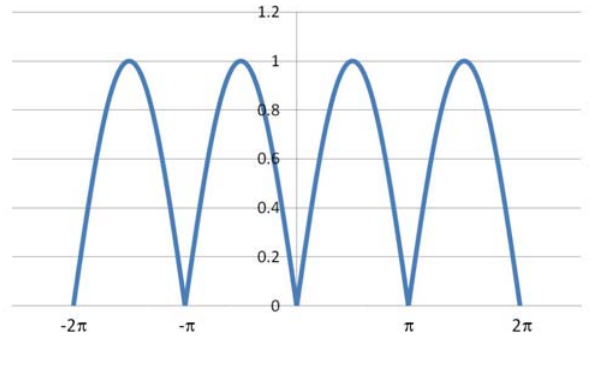
\includegraphics[width=0.5\linewidth]{figs/fig3.png} 
\item 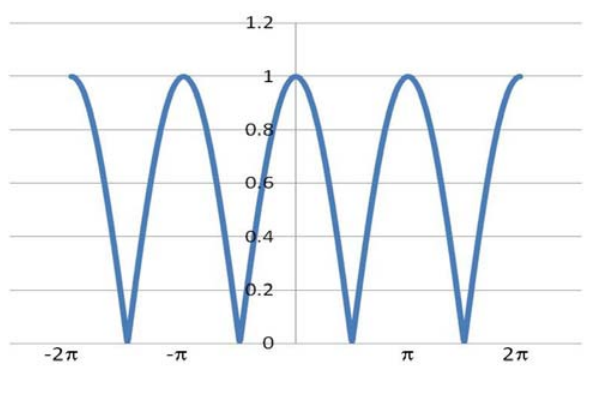
\includegraphics[width=0.5\linewidth]{figs/fig4.png} 
\end{enumerate}





\begin{align*}
    {\Large{\textbf{END OF THE QUESTION PAPER}}}
\end{align*}

\begin{align*}
    {\large{\textbf{Geology : common section}}}
\end{align*}



\begin{enumerate} VF V 

\item The first continental red beds appeared in the \_\_\_\_\_\_\_\_\_ Eon.

\hfill{\brak{\text{GATE GG 2016}}}

\begin{multicols}{4}
\begin{enumerate}
\item Proterozoic
\item Archaean
\item Hadean
\item Phanerozoic
\end{enumerate}
\end{multicols}

\item Which one of the following is a chronostratigraphic unit?

\hfill{\brak{\text{GATE GG 2016}}}

\begin{multicols}{4}
\begin{enumerate}
\item Eon
\item Period
\item Era
\item System
\end{enumerate}
\end{multicols}

\item \_\_\_\_\_\_\_\_\_ is a well-sorted sandstone containing up to 75\% quartz, with rock fragments in excess of feldspar.

\hfill{\brak{\text{GATE GG 2016}}}

\begin{multicols}{4}
\begin{enumerate}
\item Arkose
\item Lithic arenite
\item Quartz arenite
\item Feldspathic arenite
\end{enumerate}
\end{multicols}

\item International Geomagnetic Reference Field (IGRF) is used in processing regional magnetic data

\hfill{\brak{\text{GATE GG 2016}}}

\begin{multicols}{2}
\begin{enumerate}
\item to remove the secular variation of the geomagnetic field.
\item to remove the diurnal variation of the geomagnetic field.
\item to remove the latitudinal variation of the geomagnetic field.
\item to remove the terrain effect.
\end{enumerate}
\end{multicols}

\item Which one of the following layers of the Earth has the largest volume?

\hfill{\brak{\text{GATE GG 2016}}}

\begin{multicols}{4}
\begin{enumerate}
\item Upper Mantle
\item Lower Mantle
\item Outer core
\item Inner Core
\end{enumerate}
\end{multicols}

\item The S-wave shadow zone of the Earth ranges from \_\_\_\_\_\_\_\_\_.

\hfill{\brak{\text{GATE GG 2016}}}

\begin{multicols}{4}
\begin{enumerate}
\item 103° to 180°
\item 103° to 160°
\item 103° to 153°
\item 103° to 143°
\end{enumerate}
\end{multicols}

\item According to Airy’s model, gravity anomalies for fully isostatically compensated topography are characterized by

\hfill{\brak{\text{GATE GG 2016}}}


\begin{enumerate}
\item negative Bouguer anomaly and positive free-air anomaly.
\item positive Bouguer anomaly and negative free-air anomaly.
\item zero Bouguer anomaly and negative free-air anomaly.
\item positive Bouguer anomaly and zero free-air anomaly.
\end{enumerate}

\newpage


\item Match the metals (listed in Group I) with the localities of their deposits (listed in Group II).

\begin{center}
\textbf{Group I \hfill Group II} \\[6pt]
P. Iron \hfill 1. Boula \\
Q. Zinc \hfill 2. Gadag \\
R. Gold \hfill 3. Bellary \\
S. Chromium \hfill 4. Agucha \\
\end{center}

\hfill{\brak{\text{GATE GG 2016}}}

\begin{multicols}{2}
\begin{enumerate}
\item P-1; Q-2; R-3; S-4
\item P-4; Q-3; R-1; S-2
\item P-3; Q-1; R-2; S-4
\item P-3; Q-4; R-2; S-1
\end{enumerate}
\end{multicols}

\item In a region, given the palaeomagnetic inclination \brak{I\_R}, the palaeolatitude \brak{\lambda\_R} can be calculated using the formula \_\_\_\_\_\_.

\hfill{\brak{\text{GATE GG 2016}}}

\begin{multicols}{2}
\begin{enumerate}
\item $\cos \lambda\_R = \sin I\_R$
\item $\tan \lambda\_R = \tan I\_R$
\item $\tan \lambda\_R = \tfrac{1}{2}\tan I\_R$
\item $\sin \lambda\_R = 2\cos I\_R$
\end{enumerate}
\end{multicols}

\item Which one of the following parent–daughter systems has the longest half life?

\hfill{\brak{\text{GATE GG 2016}}}

\begin{multicols}{2}
\begin{enumerate}
\item $^{147}\text{Sm} \rightarrow ^{143}\text{Nd}$
\item $^{40}\text{K} \rightarrow ^{40}\text{Ar}$
\item $^{87}\text{Rb} \rightarrow ^{87}\text{Sr}$
\item $^{187}\text{Re} \rightarrow ^{187}\text{Os}$
\end{enumerate}
\end{multicols}



\item For a soil, Liquidity Index = (Natural Water Content -- X) / Plasticity Index. Here, X is ____________ .

\hfill{\brak{\text{GATE GG 2016}}}

\begin{multicols}{4}
\begin{enumerate}
\item Shrinkage Limit
\item Plastic Limit
\item Liquid Limit
\item Activity
\end{enumerate}
\end{multicols}




\item Match the following features (listed in Group I) with the different agents of erosion (listed in Group II).

\begin{tabular}{p{0.48\textwidth} p{0.48\textwidth}}
\textbf{Group I} & \textbf{Group II} \\
P. Earth pillar & 1. River \\
Q. Fjord & 2. Wind \\
R. Pot hole & 3. Glacier \\
S. Yardang & 4. Rain \\
\end{tabular}

\hfill{\brak{\text{GATE GG 2016}}}

\begin{multicols}{2}
\begin{enumerate}
\item P-2; Q-4; R-1; S-3
\item P-2; Q-3; R-4; S-1
\item P-4; Q-3; R-1; S-2
\item P-3; Q-1; R-4; S-2
\end{enumerate}
\end{multicols}

\item Match the parameters listed in Group I with the units listed in Group II.

\begin{tabular}{p{0.48\textwidth} p{0.48\textwidth}}
\textbf{Group I} & \textbf{Group II} \\
P. Hydraulic conductivity & 1. Newton sec./m\textsuperscript{2} \\
Q. Permeability & 2. m/sec \\
R. Viscosity & 3. m \\
S. Hydraulic head & 4. m\textsuperscript{2} \\
\end{tabular}

\hfill{\brak{\text{GATE GG 2016}}}

\begin{multicols}{2}
\begin{enumerate}
\item P-2; Q-4; R-1; S-3
\item P-1; Q-2; R-4; S-3
\item P-2; Q-4; R-3; S-1
\item P-4; Q-2; R-1; S-3
\end{enumerate}
\end{multicols}

\item In digital remote sensing, land–water contrast is best identified in the \_\_\_\_\_ wavelength band.

\hfill{\brak{\text{GATE GG 2016}}}

\begin{multicols}{4}
\begin{enumerate}
\item Ultraviolet
\item Near IR
\item Middle IR
\item Thermal IR
\end{enumerate}
\end{multicols}

\item Which one of the following rocks has the highest magnetic susceptibility value?

\hfill{\brak{\text{GATE GG 2016}}}

\begin{multicols}{4}
\begin{enumerate}
\item Quartzite
\item Limestone
\item Gabbro
\item Shale
\end{enumerate}
\end{multicols}





\item In which one of the following electromagnetic methods is the rate of change of secondary field recorded?

\hfill{\brak{\text{GATE GG 2016}}}


\begin{enumerate}
\item Very Low Frequency method
\item Time-domain EM method
\item Magnetotelluric method
\item TURAM method
\end{enumerate}


\item A Wenner array with 60 m spacing between current electrodes is placed over an inhomogeneous ground. If the measured potential difference and current flow in subsurface are $10 mV$ and $5 mA$, respectively, the apparent resistivity will be \_\_\_\_\_\_\_\_ Ωm. (Use \pi = 3.14)

\hfill{\brak{\text{GATE GG 2016}}}

\item Which one of the following geophysical methods is most suitable for the exploration of a horizontally stratified graphite deposit at a depth of 50 m?

\hfill{\brak{\text{GATE GG 2016}}}

\begin{multicols}{4}
\begin{enumerate}
\item Gravity
\item Magnetic
\item Radiometric
\item Electromagnetic
\end{enumerate}
\end{multicols}

\item Which one of the following logging techniques is most suitable to detect a shale layer sandwiched between two sandstone layers?

\hfill{\brak{\text{GATE GG 2016}}}

\begin{multicols}{4}
\begin{enumerate}
\item Neutron-Gamma
\item Gamma-Gamma
\item Natural Gamma
\item Sonic
\end{enumerate}
\end{multicols}

\item The following schematic diagram is a plan view of three oceanic plates forming a stable triple junction on a flat earth. Plate A subducts below Plate C normal to the plate boundary, while the contact between Plates A and B is a transform fault, as indicated. The boundary between Plates B and C is a \_\_\_\_\_\_\_\_.

\hfill{\brak{\text{GATE GG 2016}}}

\begin{figure}[h!]
    \centering
    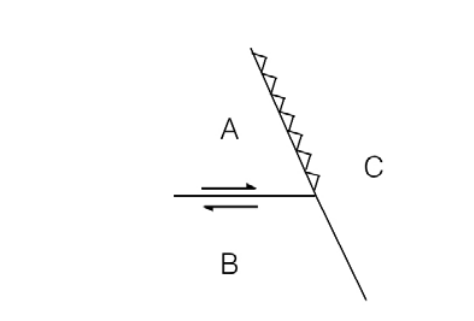
\includegraphics[width=0.4\textwidth]{figs/fig5.png}
    \caption{}
    \label{fig:q18}
\end{figure}





\begin{multicols}{2}
\begin{enumerate}
\item mid-oceanic ridge
\item subduction zone
\item sinistral transform fault
\item dextral transform fault
\end{enumerate}
\end{multicols}

\item In Gondwanaland reconstructions, much of the present west coast of India is placed adjacent to \_\_\_\_\_\_\_\_.

\hfill{\brak{\text{GATE GG 2016}}}

\begin{multicols}{4}
\begin{enumerate}
\item South America
\item Madagascar
\item Antarctica
\item Australia
\end{enumerate}
\end{multicols}

\item Two vertically dipping limbs of a fold have perpendicular strikes. The fold can be classified as \_\_\_\_\_\_\_\_.

\hfill{\brak{\text{GATE GG 2016}}}

\begin{multicols}{4}
\begin{enumerate}
\item an antiformal fold
\item a synformal fold
\item a vertical fold
\item a recumbent fold
\end{enumerate}
\end{multicols}

\item Match the crystal forms (listed in Group I) with their corresponding number of faces (listed in Group II).

\begin{tabular}{p{0.48\textwidth} p{0.48\textwidth}}
\textbf{Group I} & \textbf{Group II} \\
P. Cube & 1. Two \\
Q. Tetrahedron & 2. Four \\
R. Pinacoid & 3. Six \\
S. Dodecahedron & 4. Twelve \\
\end{tabular}

\hfill{\brak{\text{GATE GG 2016}}}

\begin{multicols}{2}
\begin{enumerate}
\item P-4; Q-2; R-3; S-1
\item P-3; Q-2; R-1; S-4
\item P-3; Q-4; R-1; S-2
\item P-1; Q-3; R-4; S-2
\end{enumerate}
\end{multicols}

\item Match the rocks in Group I with their essential mineral assemblages in Group II.

\begin{tabular}{p{0.48\textwidth} p{0.48\textwidth}}
\textbf{Group I} & \textbf{Group II} \\
P. Granodiorite & 1. Hornblende-plagioclase \\
Q. Harzburgite & 2. Plagioclase-quartz \\
R. Gabbro & 3. Olivine-orthopyroxene \\
S. Diorite & 4. Clinopyroxene-plagioclase \\
\end{tabular}

\hfill{\brak{\text{GATE GG 2016}}}

\begin{multicols}{2}
\begin{enumerate}
\item P-2; Q-3; R-4; S-1
\item P-3; Q-4; R-1; S-2
\item P-4; Q-1; R-3; S-2
\item P-1; Q-3; R-2; S-4
\end{enumerate}
\end{multicols}

\item Which one of the following mineral assemblages is stable under eclogite facies conditions?

\hfill{\brak{\text{GATE GG 2016}}}


\begin{enumerate}
\item Garnet-orthopyroxene-clinopyroxene-plagioclase
\item Garnet-clinopyroxene-plagioclase-kyanite
\item Garnet-orthopyroxene-hornblende-plagioclase
\item Garnet-clinopyroxene-kyanite-quartz
\end{enumerate}


\newpage

\begin{align*}
    {\large{\textbf{Geology(section - 1) : Optional Section}}}
\end{align*}




\item Select the CORRECT statement from the following options.

\hfill{\brak{\text{GATE GG 2016}}}


\begin{enumerate}
\item Hogback is an isolated tableland with sides that are usually steep.
\item Crevasses are deposits of glacial origin.
\item Loess comprises pebbles of rocks or minerals with some plane faces formed by wind abrasion.
\item Loamy soil is a mixture of sand and clay.
\end{enumerate}


\item Match the following patterns (listed in Group I) with their appropriate Cephalopod sutures (listed in Group II). Arrow gives the direction of aperture.

\hfill{\brak{\text{GATE GG 2016}}}

\begin{tabular}{p{0.48\textwidth} p{0.48\textwidth}}
\textbf{Group I} & \textbf{Group II} \\
P.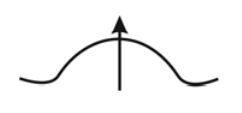
\includegraphics[width=0.5\linewidth]{figs/fig6.png}  & 1.Ceratitic \\
Q. 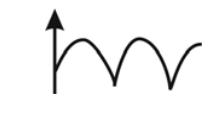
\includegraphics[width=0.5\linewidth]{figs/fig7.png}& 2.Nautilitic\\
R. 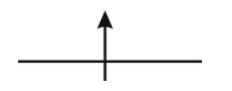
\includegraphics[width=0.5\linewidth]{figs/fig8.png} & 3. Goniatitic\\
S. 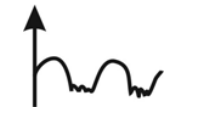
\includegraphics[width=0.5\linewidth]{figs/fig9.png} & 4.Orthoceratitic \\
\end{tabular}

\begin{enumerate}
\item P-2; Q-3; R-4; S-1
\item P-2; Q-1; R-4; S-3
\item P-4; Q-3; R-1; S-2
\item P-3; Q-1; R-4; S-2
\end{enumerate}

\item Match the following test composition (listed in Group I) with the microfossil taxa (listed in Group II).

\hfill{\brak{\text{GATE GG 2016}}}

\begin{tabular}{p{0.48\textwidth} p{0.48\textwidth}}
\textbf{Group I} & \textbf{Group II} \\
P. Organic-walled & Radiolaria  \\
Q. Siliceous & 2. Conodont  \\
R. Phosphatic & 3. Foraminifera \\
S. Calcareous  & 4. Acritarch \\
\end{tabular}


\begin{multicols}{2}
\begin{enumerate}
\item P-4; Q-3; R-1; S-2
\item P-2; Q-1; R-4; S-3
\item P-4; Q-1; R-2; S-3
\item P-3; Q-4; R-1; S-2
\end{enumerate}
\end{multicols}

\newpage

\item Which one of the following statements is CORRECT?

\hfill{\brak{\text{GATE GG 2016}}}


\begin{enumerate}
\item Movement of the shoreline seaward is transgression.
\item No movement of the shoreline is transgression.
\item Movement of the shoreline seaward as a result of sea-level fall is forced regression.
\item Movement of the shoreline landward is regression.
\end{enumerate}


\item Mud-supported limestone containing greater than 10\% allochems is called _____________.

\hfill{\brak{\text{GATE GG 2016}}}

\begin{multicols}{4}
\begin{enumerate}
\item Packstone
\item Wackestone
\item Grainstone
\item Mudstone
\end{enumerate}
\end{multicols}

\item At a depth of 500 m, the determined in-situ stresses in a rock mass are as follows: maximum horizontal stress = 20 MPa, minimum horizontal stress = 8 MPa and vertical stress = 13.5 MPa. Assuming the principal stress directions to be vertical and horizontal, if this compressive stress field leads to faulting, the plausible fault type would be __________.

\hfill{\brak{\text{GATE GG 2016}}}

\begin{multicols}{2}
\begin{enumerate}
\item Normal fault
\item Reverse fault
\item Strike-slip fault
\item Detachment fault
\end{enumerate}
\end{multicols}

\item The following litholog represents fossil occurrences (figure). The biostratigraphic zone represented by the assemblage is.

\hfill{\brak{\text{GATE GG 2016}}}

\begin{figure}[h!]
    \centering
    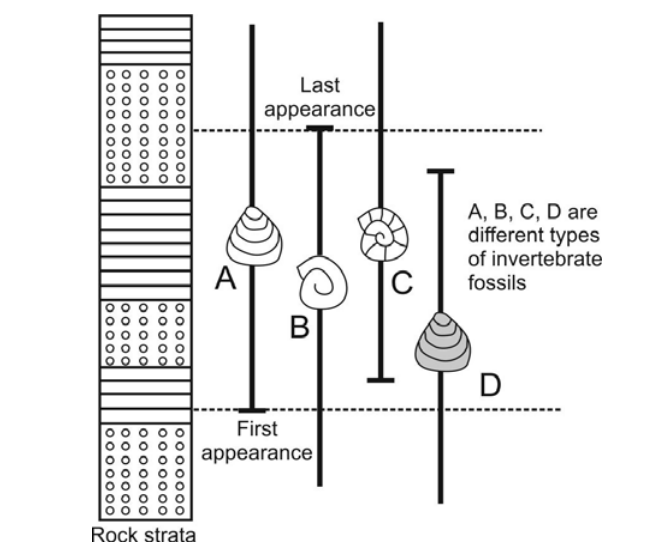
\includegraphics[width=0.4\textwidth]{figs/fig10.png}
    \caption{}
    \label{fig:q18}
\end{figure}


\begin{multicols}{2}
\begin{enumerate}
\item Assemblage Zone
\item Taxon Range Zone
\item Consecutive Range Zone
\item Acme Zone
\end{enumerate}
\end{multicols}

\item Which one of the following stratigraphic successions is in the correct chronological order (oldest at bottom)?

\hfill{\brak{\text{GATE GG 2016}}}


\begin{enumerate}
\item  Iron Ore Group, Older Metamorphic Group, Kolhan Group
\item Chitradurga Group, Sargur Group, Bababudan Group 

\item  Jharol Group, Alwar Group, Ajabgarh Group 
\item  Chitravati Group, Papaghni Group, Kurnool Group 
\end{enumerate}


\item Water content is 10\%, total porosity is 25\% and specific gravity of solid grains is 2.5. The volume of water required to be added to 100 $m\textsuperscript{3}$ of the wet soil to make it fully saturated is __________ $m\textsuperscript{3}$.

\hfill{\brak{\text{GATE GG 2016}}}

% (NAT question — no options)

\item In a zone of superposed folding, poles to bedding plot as a great circle on the stereonet. For such a case, the fold axes related to the first generation of folds will:

\hfill{\brak{\text{GATE GG 2016}}}

\begin{multicols}{2}
\begin{enumerate}
\item be parallel to the great circle.
\item lie on the great circle at its intersections with the primitive circle.
\item lie at the poles to the great circle.
\item be randomly distributed.
\end{enumerate}
\end{multicols}

\item For horizontal flow in a fully saturated aquifer, the product of hydraulic conductivity and aquifer thickness is called the __________.

\hfill{\brak{\text{GATE GG 2016}}}

\begin{multicols}{2}
\begin{enumerate}
\item specific yield
\item transmissivity
\item coefficient of storage
\item seepage force
\end{enumerate}
\end{multicols}

\item If a rectangle is deformed into a parallelogram of equal area by simple shear deformation (with shear strain $\gamma$) parallel to the abscissa, the displacement matrix is _______________.

\hfill{\brak{\text{GATE GG 2016}}}

\begin{multicols}{1}
\begin{enumerate}
\item $\begin{pmatrix}1 & \gamma \\ 0 & 1\end{pmatrix}$
\item $\begin{pmatrix}1 & 0 \\ \gamma & 1\end{pmatrix}$
\item $\begin{pmatrix}1 & 0 \\ 0 & 1\end{pmatrix}$
\item $\begin{pmatrix}0 & \gamma \\ 1 & 0\end{pmatrix}$
\end{enumerate}
\end{multicols}

\item If tangent Young's modulus (at 50\% of the uniaxial compressive strength) and modulus ratio of a rock are given as 60 GPa and 500, respectively, the uniaxial compressive strength of the rock is ________ MPa.

\hfill{\brak{\text{GATE GG 2016}}}

% (NAT question — no options)

\item In a rock sample, the values of $(^{87}\mathrm{Sr}/^{86}\mathrm{Sr})_{\text{present}}$ and $(^{87}\mathrm{Rb}/^{86}\mathrm{Sr})_{\text{present}}$ are 0.7125 and 0.2, respectively. The decay constant $\lambda$ of $^{87}\mathrm{Rb}$ is $1.42\times10^{-11}\ \text{year}^{-1}$, and time before present $t$ is 1000 million years. The value of the initial ratio $(^{87}\mathrm{Sr}/^{86}\mathrm{Sr})_0$ is ________.

\hfill{\brak{\text{GATE GG 2016}}}

% (NAT question — no options)

\item The $\Delta G^0$ of the reaction $2\,\mathrm{Fe_3O_4} + 0.5\,\mathrm{O_2} = 3\,\mathrm{Fe_2O_3}$ at 300°C and 500 bars is $-40.657$ kilocalories. The value of $\log f_{\mathrm{O}_2}$ at that temperature and pressure is ______________.

\hfill{\brak{\text{GATE GG 2016}}}

% (NAT question — no options)

\item Match the types of mineralization in Group-I with their appropriate tectonic settings in Group-II. (VMS = volcanogenic massive sulfide)

\hfill{\brak{\text{GATE GG 2016}}}
\begin{tabular}{p{0.48\textwidth} p{0.48\textwidth}}
\textbf{Group I} & \textbf{Group II} \\
P. Cyprus-type VMS & 1.Island Arc  \\
Q. Kuroko-type VMS & 2. Continental Arc \\
R. Porphyry copper & 3. Intraplate\\
S. Diamond in Kimberlite  & 4.  Mid Oceanic Ridge  \\
\end{tabular}



\begin{multicols}{2}
\begin{enumerate}
\item P-1; Q-2; R-3; S-4
\item P-4; Q-1; R-2; S-3
\item P-4; Q-2; R-3; S-1
\item P-2; Q-1; R-4; S-3
\end{enumerate}
\end{multicols}

\item Clay minerals and Fe-oxide minerals, products of hydrothermal alteration and supergene oxidation, are good indicators of mineralization. Choose the CORRECT Thematic Mapper (TM) band ratio images for detection of these minerals.

\hfill{\brak{\text{GATE GG 2016}}}


\begin{enumerate}
\item band ratio 5/7 for clay and 3/1 for Fe-oxide minerals
\item band ratio 3/1 for clay and 5/7 for Fe-oxide minerals
\item band ratio 3/7 for clay and 5/1 for Fe-oxide minerals
\item band ratio 5/1 for clay and 3/7 for Fe-oxide minerals
\end{enumerate}


\item The age range of reservoir rock in Cambay oil field is _______________.

\hfill{\brak{\text{GATE GG 2016}}}

\begin{multicols}{2}
\begin{enumerate}
\item 34 – 15 million years
\item 56 – 34 million years
\item 65 – 56 million years
\item 100 – 65 million years
\end{enumerate}
\end{multicols}

\item Which one of the following statements is CORRECT in all respects for the amphibole glaucophane, Na\textsubscript{2}Mg\textsubscript{3}Al\textsubscript{2}Si\textsubscript{8}O\textsubscript{22}(OH)\textsubscript{2}?

\hfill{\brak{\text{GATE GG 2016}}}


\begin{enumerate}
\item Na is in the M4-site, Al is in octahedral coordination and Si is in tetrahedral coordination.
\item Na is in the A-site, both Al and Si are in tetrahedral coordination.
\item Na is in the M4-site, Al is partly in octahedral and partly in tetrahedral coordination, Si is in tetrahedral coordination.
\item Na is in the A-site, both Al and Si are in octahedral coordination.
\end{enumerate}


\item Choose the CORRECT modern analog of Besshi type VMS deposits (all are ocean floor rift zones).

\hfill{\brak{\text{GATE GG 2016}}}

\begin{multicols}{2}
\begin{enumerate}
\item 21°N East Pacific Rise (EPR)
\item Guaymas Basin
\item Lau Basin
\item Trans Atlantic Geotraverse (TAG)
\end{enumerate}
\end{multicols}

\item Which one of the following options is arranged in the CORRECT increasing order of Vicker's micro-hardness?

\hfill{\brak{\text{GATE GG 2016}}}

\begin{multicols}{2}
\begin{enumerate}
\item galena < chalcopyrite < sphalerite < magnetite
\item sphalerite < galena < magnetite < chalcopyrite
\item galena < magnetite < chalcopyrite < sphalerite
\item sphalerite < magnetite < chalcopyrite < galena
\end{enumerate}
\end{multicols}

\item The $(^{18}\mathrm{O}/^{16}\mathrm{O})$ of a quartz sample yields a value of 0.0019. The value of $\delta^{18}\mathrm{O}$ of the quartz sample is _________.   (Use the value of the ratio in VSMOW as 0.002005.) 

\hfill{\brak{\text{GATE GG 2016}}}

% (NAT question — no options)

\item The ionic strength of a solution having 0.5 molal NaCl and 0.25 molal CaCl\textsubscript{2} is _________ molal.

\hfill{\brak{\text{GATE GG 2016}}}

% (NAT question — no options)

\item During which stage of coalification is most of the methane gas generated?

\hfill{\brak{\text{GATE GG 2016}}}

\begin{multicols}{4}
\begin{enumerate}
\item Lignite
\item Peat
\item Bituminous
\item Anthracite
\end{enumerate}
\end{multicols}

\item The figure shows the liquidus phase relations in the forsterite–anorthite–silica system at 1 bar pressure. From the options below, identify the CORRECT reaction that takes place at the isobaric invariant point P.

\hfill{\brak{\text{GATE GG 2016}}}

\begin{figure}[h!]
    \centering
    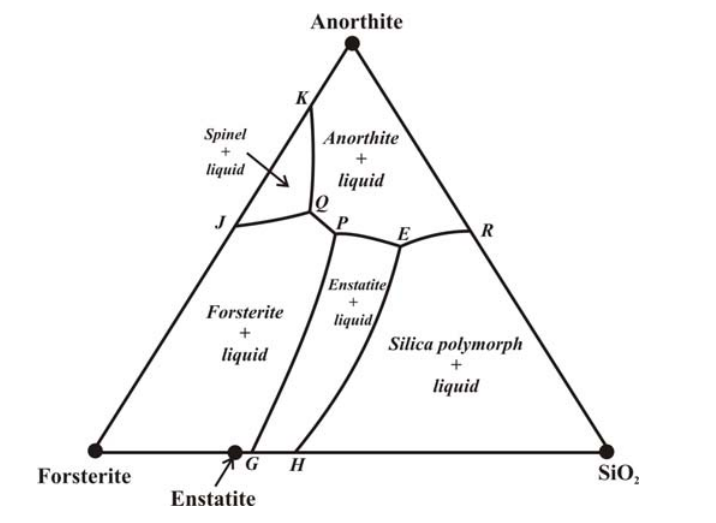
\includegraphics[width=0.4\textwidth]{figs/fig11.png}
    \caption{}
    \label{fig:q18}
\end{figure}



\begin{enumerate}
\item Liquid (at P) = Forsterite + Anorthite + Enstatite
\item Liquid (at P) + Forsterite = Anorthite + Enstatite
\item Liquid (at P) + Forsterite + Anorthite = Enstatite
\item Liquid (at P) = Forsterite + Anorthite + Silica polymorph
\end{enumerate}


\item A garnet peridotite contains 2400 ppm of nickel. After 20\% partial melting, a basaltic melt is generated, leaving a residue comprising 60\% olivine, 30\% orthopyroxene and 10\% clinopyroxene. Given the partition coefficients $K_D$ (Ni) as: olivine = 10, orthopyroxene = 4, clinopyroxene = 2, the nickel concentration in the melt, assuming equilibrium batch melting, is  ppm.

\hfill{\brak{\text{GATE GG 2016}}}



\item Which one of the following mineral assemblages is stable in a pelitic rock in the greenschist facies?

\hfill{\brak{\text{GATE GG 2016}}}

\begin{multicols}{2}
\begin{enumerate}
\item Albite-epidote-actinolite-chlorite-quartz
\item Muscovite-biotite-garnet-quartz
\item Tremolite-talc-calcite-quartz
\item Muscovite-biotite-garnet-sillimanite-quartz
\end{enumerate}
\end{multicols}

\item Match the co-existing mineral pairs in Group I with the diagnostic metamorphic conditions they are associated with in Group II.

\begin{tabular}{p{0.48\textwidth} p{0.48\textwidth}}
\textbf{Group I} & \textbf{Group II} \\
P. Talc-phengite & 1. Ultrahigh temperature \\
Q. Cordierite-andalusite & 2. Very low temperature \\
R. Spinel-quartz & 3. Ultrahigh pressure \\
S. Laumontite-wairakite & 4. Low pressure, high temperature \\
\end{tabular}

\hfill{\brak{\text{GATE GG 2016}}}

\begin{multicols}{2}
\begin{enumerate}
\item P-2; Q-3; R-1; S-4
\item P-3; Q-4; R-1; S-2
\item P-4; Q-1; R-2; S-3
\item P-3; Q-2; R-4; S-1
\end{enumerate}
\end{multicols}

\newpage


\item Out of the following symmetry elements, which one is present in all classes of the cubic system?

\hfill{\brak{\text{GATE GG 2016}}}


\begin{enumerate}
\item Four axes of 3-fold symmetry
\item Three axes of 4-fold symmetry
\item Six axes of 2-fold symmetry
\item Three mirror planes
\end{enumerate}


\item Match the minerals in Group-I with their optical properties in Group-II.

\begin{tabular}{p{0.48\textwidth} p{0.48\textwidth}}
\textbf{Group I} & \textbf{Group II} \\
P. Calcite & 1. Uniaxial negative, low birefringence, high relief \\
Q. Nepheline & 2. Uniaxial negative, high birefringence, moderately high relief \\
R. Apatite & 3. Uniaxial positive, low birefringence, low relief \\
S. Quartz & 4. Uniaxial negative, low birefringence, low relief \\
\end{tabular}

\hfill{\brak{\text{GATE GG 2016}}}

\begin{multicols}{2}
\begin{enumerate}
\item P-4; Q-2; R-1; S-3
\item P-3; Q-2; R-4; S-1
\item P-2; Q-4; R-1; S-3
\item P-1; Q-3; R-2; S-4
\end{enumerate}
\end{multicols}



\begin{align*}
    {\large{\textbf{Section 2 (Geophysics): Optional Section}}}
\end{align*}








\item Depth migration is applied to a stacked seismic section. Compared to the stacked section, dipping events in the migrated section

\hfill{\brak{\text{GATE GG 2016}}}


\begin{enumerate}[label=(\Alph*)]
\item have a steeper slope and move updip.
\item remain unchanged.
\item have a gentler slope and move downdip.
\item have a steeper slope and move downdip.
\end{enumerate}

\item A monochromatic elastic wave of frequency 20 Hz propagates in a medium with average velocity 3 km/s. For zero offset reflection from horizontal reflectors, the thickness of the vertical first Fresnel zone is \underline{\hspace{3cm}} m.

\hfill{\brak{\text{GATE GG 2016}}}

\item The following figure shows a seismic reflection experiment above a reflector that dips $45^\circ$. The P-wave velocity in the medium is constant and equal to 2 km/s. The source is kept at location `S' and the receiver is kept at location `G'. The midpoint between S and G is denoted by `M' and the depth to the reflector from `M' is 1 km. The traveltime of the primary reflected arrival recorded at the receiver is equal to \underline{\hspace{3cm}} seconds.

\hfill{\brak{\text{GATE GG 2016}}}

\begin{figure}[h]
\centering
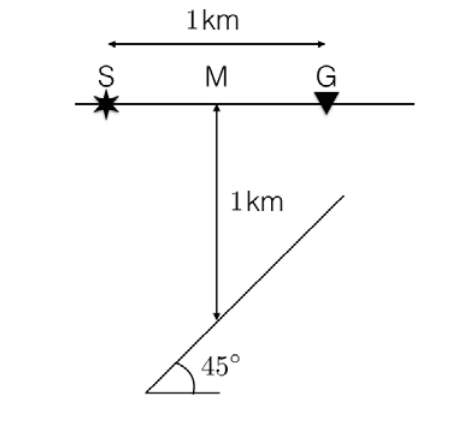
\includegraphics[width=0.2\textwidth]{figs/fig12.png}
\caption{}
\label{fig q28}
\end{figure}



\newpage

\item Given a seismic wavelet $w=\{6,-4,-2\}$ and reflectivity series $r=\{0,1,0\}$, the corresponding seismic trace is \underline{\hspace{3cm}}.

\hfill{\brak{\text{GATE GG 2016}}}

\begin{multicols}{4}
\begin{enumerate}[label=(\Alph*)]
\item $\{0,-4,0,0,0\}$
\item $\{0,-2,-4,6,0\}$
\item $\{0,6,0,0,0\}$
\item $\{0,6,-4,-2,0\}$
\end{enumerate}
\end{multicols}

\item The time period of the signal $s(t)=\sin(3\pi t)+\cos(2\pi t)$ is \underline{\hspace{3cm}} seconds.

\hfill{\brak{\text{GATE GG 2016}}}

\item Assertion (a): The inverse of a minimum phase wavelet is causal and stable.

Reason (r): The $Z$-transform of a minimum phase wavelet has all its zeros outside the unit circle.

\hfill{\brak{\text{GATE GG 2016}}}


\begin{enumerate}[label=(\Alph*)]
\item (a) is true but (r) is false
\item (a) is false but (r) is true
\item Both (a) and (r) are true and (r) is the correct reason for (a)
\item Both (a) and (r) are true and (r) is not the correct reason for (a)
\end{enumerate}


\item The value of free-air correction (assuming sea level as datum plane) at an elevation of 150 m is \underline{\hspace{3cm}} mGal.

\hfill{\brak{\text{GATE GG 2016}}}

\item A spherical cavity of radius 8 m has its centre 15 m below the surface. If the cavity is full of sediments of density $1.5\times10^{3}\,\mathrm{kg/m^3}$ and is in a rock body of density $2.4\times10^{3}\,\mathrm{kg/m^3}$, the maximum value of its gravity anomaly is \underline{\hspace{3cm}} mGal.

\hfill{\brak{\text{GATE GG 2016}}}

\item Match the items (listed in Group I) with the corresponding corrections applied for reduction of marine gravity data (listed in Group II).

\hfill{\brak{\text{GATE GG 2016}}}

\noindent Group I

P. Effect of rotating homogeneous ellipsoidal Earth

Q. Effect of deficit mass from mean sea level to average depth to ocean floor

R. Effect of relative motion of ship with respect to revolving Earth

S. Effect of elastic creep of gravimeter spring system and Earth tides

\noindent Group II

1. Drift correction

2. Latitude correction

3. Bouguer correction

4. Eotvos correction

\begin{multicols}{2}
\begin{enumerate}[label=(\Alph*)]
\item P-4; Q-3; R-1; S-2
\item P-2; Q-3; R-4; S-1
\item P-4; Q-1; R-2; S-3
\item P-3; Q-1; R-4; S-2
\end{enumerate}
\end{multicols}

\item Which one of the following Natural Remanent Magnetization (NRM) gives a primary, stable magnetization for igneous rocks?

\hfill{\brak{\text{GATE GG 2016}}}


\begin{enumerate}[label=(\Alph*)]
\item Depositional Remanent Magnetization (DRM)
\item Thermo Remanent Magnetization (TRM)
\item Chemical Remanent Magnetization (CRM)
\item Isothermal Remanent Magnetization (IRM)
\end{enumerate}


\item The following figure shows the total magnetic field intensity anomaly above a spherical body polarized by the present day geomagnetic field. From among the options below, identify the region in which such an anomaly could be observed.

\begin{figure}[h]
\centering
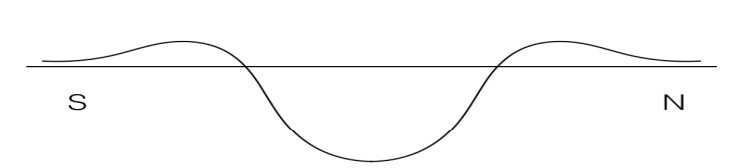
\includegraphics[width=0.6\textwidth]{figs/fig13.png}
\caption{}
\label{fig:q36}
\end{figure}

\hfill{\brak{\text{GATE GG 2016}}}

\begin{multicols}{4}
\begin{enumerate}[label=(\Alph*)]
\item Equator
\item Latitude $27^\circ$
\item North pole
\item South pole
\end{enumerate}
\end{multicols}

\item Which one of the following is the ray path for the P-wave that converts to S-wave while passing through the solid inner core?

\hfill{\brak{\text{GATE GG 2016}}}

\begin{multicols}{4}
\begin{enumerate}[label=(\Alph*)]
\item PKiKP
\item PKIKP
\item pPcP
\item PKJKP
\end{enumerate}
\end{multicols}

\item Which one of the following statements is CORRECT for the stress drop ($\Delta\sigma$) of an earthquake?

\hfill{\brak{\text{GATE GG 2016}}}


\begin{enumerate}[label=(\Alph*)]
\item Large slip on a small fault will cause more stress drop.
\item Small slip on a large fault will cause more stress drop.
\item Stress drop is inversely proportional to the slip of the fault.
\item Stress is directly proportional to the rupture dimension.
\end{enumerate}


\item The energy released by an earthquake of magnitude 7 is \underline{\hspace{3cm}} times the energy released by an earthquake of magnitude 4 (use Kanamori's formula).

\hfill{\brak{\text{GATE GG 2016}}}

\item In resistivity logging using a `Normal device', the distance between electrodes A and M is 0.40 m. If 20 mA current generates 10 mV potential, the apparent resistivity of the layer between the electrodes is \underline{\hspace{3cm}} $\Omega$m. (Use $\pi=3.14$)

\hfill{\brak{\text{GATE GG 2016}}}

\item A cylindrical sandstone core sample of diameter 0.02 m and length 0.04 m is fully saturated with brine solution of resistivity 0.5 $\Omega$m. The resistance of the saturated sample measured in the laboratory is 500 $\Omega$. The formation factor of the sample is \underline{\hspace{3cm}}. (Use $\pi=3.14$)

\hfill{\brak{\text{GATE GG 2016}}}

\item A Schlumberger array with current electrode separation 50 m and potential electrode separation 5 m is placed over an inhomogeneous medium. If the measured potential difference is 50 mV and the computed apparent resistivity is 100 $\Omega$m, then the magnitude of current passing through the subsurface is \underline{\hspace{3cm}} mA. (Use $\pi=3.14$)

\hfill{\brak{\text{GATE GG 2016}}}

\item Two horizontal layers have resistivities and thicknesses of 10 $\Omega$m, 5 m and 50 $\Omega$m, 10 m, respectively. If the two layers are reduced to a single layer, then the coefficient of electrical anisotropy will be \underline{\hspace{3cm}}.

\hfill{\brak{\text{GATE GG 2016}}}

\newpage

\item The five-layer Schlumberger resistivity sounding curve given below represents \underline{\hspace{3cm}}.


\hfill{\brak{\text{GATE GG 2016}}}

\begin{figure}[h]
\centering
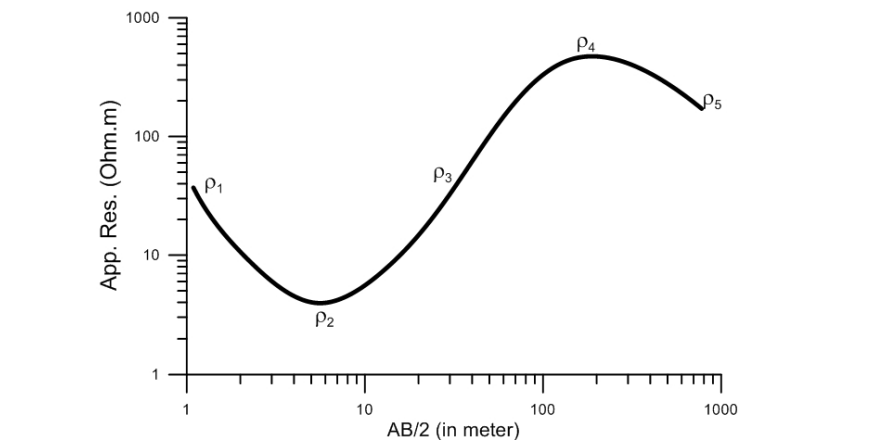
\includegraphics[width=0.6\textwidth]{figs/fig14.png}
\caption{}
\label{fig:q44}
\end{figure}



\begin{multicols}{4}
\begin{enumerate}[label=(\Alph*)]
\item HAQ-type
\item HKQ-type
\item HKH-type
\item HAK-type
\end{enumerate}
\end{multicols}



\item How are the numerical values of the real and imaginary components of the impedance tensor ($Z$) in Magnetotelluric (MT) method related over a homogeneous half-space?

\hfill{\brak{\text{GATE GG 2016}}}


\begin{enumerate}[label=(\Alph*)]
\item Imaginary component is one third of the real component.
\item Imaginary component is half of the real component.
\item Imaginary component is equal to the real component.
\item Imaginary component is twice that of the real component.
\end{enumerate}


\item The strike of a 2-D geological structure is in Y-direction. From the following options, choose the field components required to compute the apparent resistivity in E-Polarization mode for plane wave electromagnetic signals.

\hfill{\brak{\text{GATE GG 2016}}}

\begin{multicols}{4}
\begin{enumerate}[label=(\Alph*)]
\item $E_x$ and $H_x$
\item $E_x$ and $H_y$
\item $E_y$ and $H_y$
\item $E_y$ and $H_x$
\end{enumerate}
\end{multicols}

\item Dip angle electromagnetic methods are suitable to delineate

\hfill{\brak{\text{GATE GG 2016}}}


\begin{enumerate}[label=(\Alph*)]
\item both vertical and horizontal conductors.
\item horizontal conductors only.
\item vertical and dipping conductors.
\item horizontal and dipping conductors.
\end{enumerate}


\item Which one of the following equations is CORRECT for a time invariant field?

\hfill{\brak{\text{GATE GG 2016}}}

\begin{multicols}{2}
\begin{enumerate}[label=(\Alph*)]
\item $\nabla\times\mathbf{E}=0$
\item $\nabla\cdot\mathbf{B}=0$
\item $\nabla\times\mathbf{H}=\mathbf{J}+\dfrac{\partial\mathbf{D}}{\partial t}$
\item $\nabla\times\mathbf{H}=\mathbf{J}$
\end{enumerate}
\end{multicols}

\newpage

\item The solution to the Laplace equation $\nabla^2 \Phi =0$ in a spherical coordinate system with spherical symmetry is \underline{\hspace{3cm}}. $A$ and $B$ are constants and $r$ is the distance of the observation point from the source.

\hfill{\brak{\text{GATE GG 2016}}}

\begin{multicols}{4}
\begin{enumerate}[label=(\Alph*)]
\item $\displaystyle \Phi(r)=\dfrac{A}{r^2}$
\item $\displaystyle \Phi(r)=A+\dfrac{B}{r}$
\item $\displaystyle \Phi(r)=A\ln r+B$
\item $\displaystyle \Phi(r)=Ar+\dfrac{B}{r}$
\end{enumerate}
\end{multicols}

\item If $J$ is the Jacobian matrix in a geophysical inverse problem, then the addition of the regularization parameter, $\lambda$, as $J^TJ + \lambda I$, in finding the inverse leads to

\hfill{\brak{\text{GATE GG 2016}}}


\begin{enumerate}[label=(\Alph*)]
\item unstable solution with increased parameter resolution
\item stable solution with increased parameter resolution
\item unstable solution with decreased parameters resolution
\item stable solution with decreased parameter resolution
\end{enumerate}


\item The Singular Value Decomposition of a square nonsingular matrix $J$ is given by $J=U\Sigma V^{T}$. The inverse of matrix $J$ will be

\hfill{\brak{\text{GATE GG 2016}}}

\begin{multicols}{1}
\begin{enumerate}[label=(\Alph*)]
\item $J^{-1}=U\Sigma^{-1}V^{T}$
\item $J^{-1}=V\Sigma^{-1}U^{T}$
\item $J^{-1}=V\Sigma U^{T}$
\item $J^{-1}=U\Sigma V^{T}$
\end{enumerate}
\end{multicols}

\item The fraction of a radioactive nuclide remaining after 10 half-lives is closest to

\hfill{\brak{\text{GATE GG 2016}}}

\begin{multicols}{4}
\begin{enumerate}[label=(\Alph*)]
\item $0.1$
\item $0.01$
\item $0.001$
\item $0.0001$
\end{enumerate}
\end{multicols}

\item The correct relationship between the residual amount $P$ of the parent radionuclide and amount $D$ of the daughter product in a radioactive decay is

\hfill{\brak{\text{GATE GG 2016}}}

\begin{multicols}{2}
\begin{enumerate}[label=(\Alph*)]
\item $D=P_0-P$
\item $P=P_0-D$
\item $D=P\left(e^{\lambda t}-1\right)$
\item $P=P_0e^{-\lambda t}$
\end{enumerate}
\end{multicols}

\item Which one of the following resistivity sounding curves exhibits both `Equivalence' and `Suppression' type ambiguities in interpretation of data?

\hfill{\brak{\text{GATE GG 2016}}}


\begin{enumerate}[label=(\Alph*)]
\item HA-type
\item AH-type
\item HK-type
\item KH-type
\end{enumerate}


\newpage

\item For land seismic data acquisition, the following figure is a schematic plot of arrival times of seismic waves recorded at several detectors placed along the $x$-axis. The shot is placed at the origin $(x=0)$. (Match the events labelled in the figure listed in Group I with their corresponding types listed in Group II.)

\begin{figure}[h]
\centering
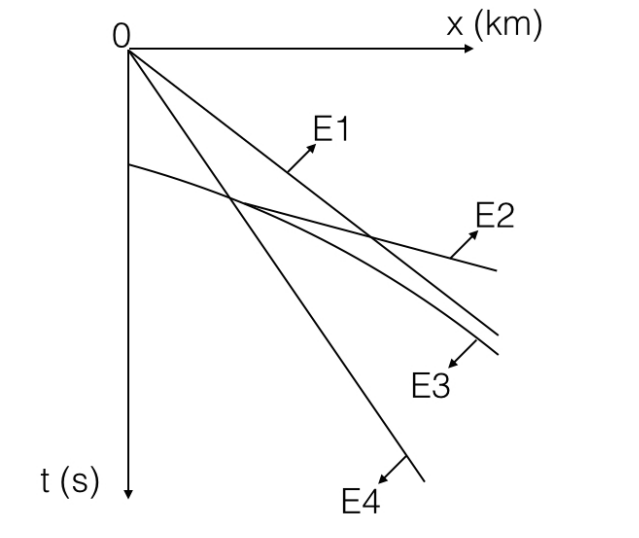
\includegraphics[width=0.6\textwidth]{figs/fig15.png}
\caption{}
\label{fig:q55}
\end{figure}

\hfill{\brak{\text{GATE GG 2016}}}

\begin{tabular}{p{0.48\textwidth} p{0.48\textwidth}}
\textbf{Group I} & \textbf{Group II} \\
P. E1 & 1. Ground roll \\
Q. E2 & 2. Direct arrival \\
R. E3& 3. Refracted energy \\
S. E4 & 4. Primary reflection\\
\end{tabular}
\begin{enumerate}[label=(\Alph*)]
\item P-3; Q-1; R-2; S-4
\item P-2; Q-3; R-4; S-1
\item P-1; Q-4; R-3; S-2
\item P-4; Q-2; R-1; S-3
\end{enumerate}




\begin{align*}
 {\LARGE{\textbf{END OF THE QUESTION PAPER}}}
\end{align*}


\end{enumerate}


\end{document}






